\chapter{Introduction}
\section{What are blockchains}
Blockchain is a bit different from other subjects, in the sense that it needs to be first defined. It is remarkable and so many people try to define it in their own way. Our definition of blockchain is as follows :
\dfn{Blockchain}{Blockchains are the technology underlying \textbf{\underline{decentralized} \underline{digital trust} \underline{platforms}}.}

\subsection*{Decentralized system}
A decentralized system is one where no single entity (person/company)
is responsible for the smooth operation of the system. Indeed, blockchains are peer-to-peer systems,
where each peer has the same prescribed behavior; no peer is unique. Peers communicate with each
other by exchanging messages. Beyond this message exchange, peers function independently of one
another.

\subsection*{Trust}
Trust is a medium that drives human interactions. Human success is based on flexible cooperation in large numbers. This requires trust. The underlying mechanism of trust dictates how large the size of human cooperation can get. 
\subsubsection*{Types of trust}
\begin{itemize}
    \item \textbf{Tribal Trust :} \\
    Tribal trust is the traditional version of trust. People who shared similarities in language, generics compositions, and customs, organized themselves around tribal societies. It was not very scaled in number or geographical place and was rather local. 
    \item  \textbf{Institutional Trust :} \\
    Since the end of WWII, the dominant human organization has been institutional. The underlying mechanism of trust is a set of laws and transparent and rigorous enforcement of the law. “No one is above the law”.\\
    This notion of trust has enabled human societies to cooperate on a global scale. It was extended to every aspect of human activity, travel, commerce, and communication.\\
    However, the drawback is that the institutions are centralized, and the power to enforce and promulgate the laws is concentrated in the hands of a few individuals. The concentration of power leads to unintended consequences, including corruptibility, autocratic tendencies, and rent-seeking.
    \item \textbf{Distributed trust :} \\
    The siren song of blockchains is that the scaling and flexibility of institutional
    trust are possible without its negative aspects, i.e., the creation of a decentralized trust
    system. This is where blockchains play a significant role. \\
    Blockchains are guaranteed to be secure even if some fraction of peers act maliciously. The
    only requirement is that sufficiently many peers operate according to the prescribed behavior. This
    is called the honest majority assumption. Thus, any user of a blockchain does not need to trust
    all peers in the system or even one particular peer. Instead, it just needs to trust that a majority
    of peers are honest. This is a key feature of blockchains that are not present in other peer-to-peer
    systems, or indeed, any other system.
\end{itemize}
\begin{figure}
    \centering
    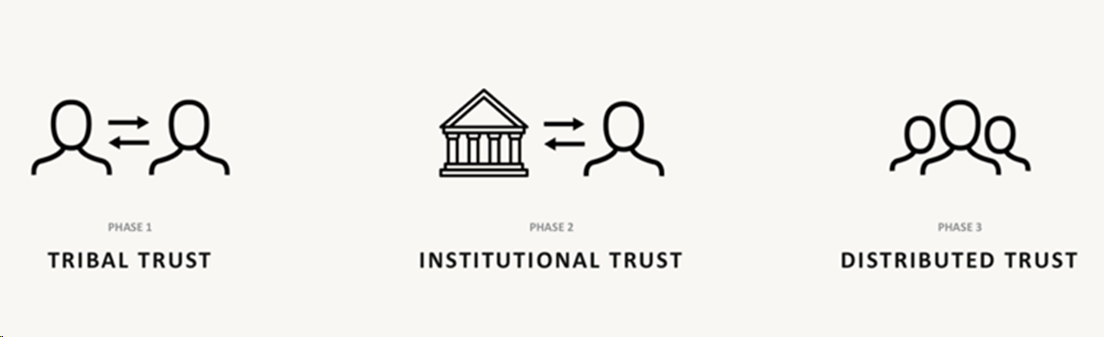
\includegraphics[width=0.7\linewidth]{Fig/01/F1}
    \caption{Evolution of Trust over human history}
    \label{fig:f1}
\end{figure}

\subsection*{Digital platforms}
Digital platforms are marketplaces where suppliers and consumers come together and trade. A digital platform is one in which two (or more) parties interact, and some transaction takes place. There are many examples of digital platforms today. For example, Amazon/eBay is a platform for the exchange of goods. It provides a place where sellers can list goods that they are selling, and buyers can choose to buy any listed goods. Among other things, the
platform ensures that the transaction takes place securely. It also handles disputes in transactions. Other examples of platforms are Uber/Lyft (for rides), AirBnB (for temporary accommodation), etc. Digital platforms have played a significant role in the global economy in the last decade. For the last decade and beyond, platform companies have been the dominant force in the economy. Here, we put the top six companies by market cap. They're all platform companies. 
\begin{figure}[h!]
    \centering
    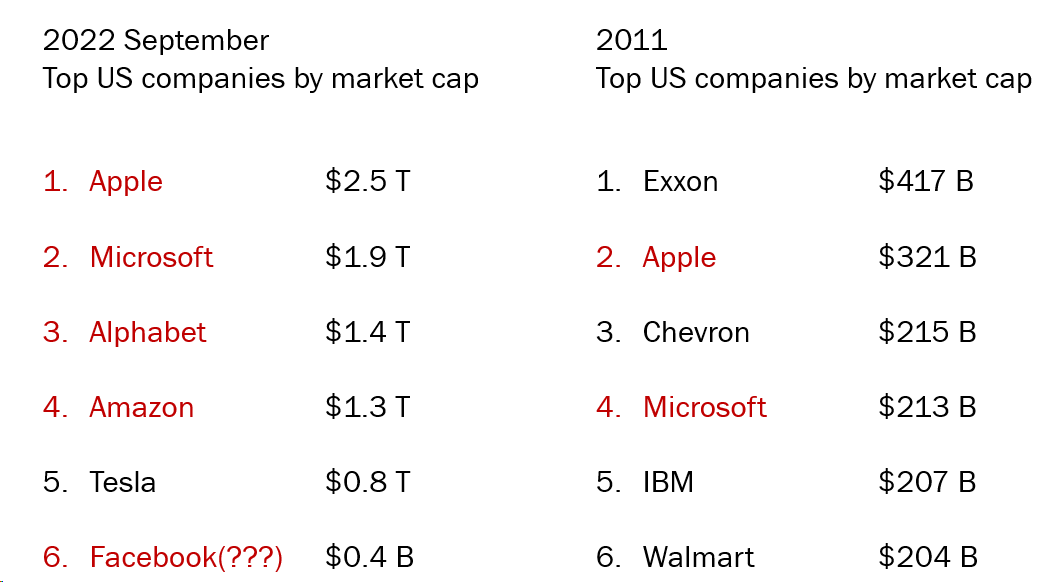
\includegraphics[width=0.7\linewidth]{Fig/01/F4}
    \caption{Evolution of Trust over human history}
    \label{fig:f4}
\end{figure}    
The aforementioned digital platforms are not truly decentralized in the sense, they do not offer distributed trust. By using any platform, we implicitly trust the (single) company behind that platform to handle transactions faithfully. The platform holds much power in arbitrating disputes. It can also arbitrarily decide the fees to charge for the service. (Of course, the reputation/popularity of the platform is at stake, which prevents it from behaving arbitrarily).\\\\
Blockchains hold the promise to decentralize the digital platforms we see today. From a user’s perspective, the platform’s functionality will be identical. However, the platform will no longer be operated by a single company but rather by a multitude of small stakeholders, each running the same blockchain code. The ‘trust’ factor in the system becomes distributed.

\section{Bitcoin as the first blockchain}
The term Blockchain was introduced in late 2008 with the advent of Bitcoin. The inventor of Bitcoin is Satoshi Nakamoto, a pseudonym for the person or persons who developed the cryptocurrency, authored the Bitcoin white paper and created and deployed the original Bitcoin software. Bitcoin is a cryptocurrency: a decentralized, digital payment platform. As such, cryptocurrencies are one of the simplest applications of blockchains. Today, there is a multitude of blockchain designs for cryptocurrencies and other applications. However, they all retain many of the core design components that were
introduced in Bitcoin. Thus, the term ‘blockchain’ has remained in all of them.\\\\
Bitcoin is among many attempts in history to create a decentralized, digital payment platform (the term ‘currency’ is to be thought of as a ‘token’ that is used on this payment platform). Unlike all previous attempts, Bitcoin has stood the test of time. Its popularity, which can be measured by its price in dollars, has grown manyfold over the twelve years since its introduction.\\\\
It may seem that the fall and rise in the price of Bitcoin is a bubble, but based on Figure \ref{fig:f2}, the red graph that shows the changes in the price of Bitcoin says that the price of Bitcoin has gone up and down, but other bubbles burst at once and their prices do not rise much. This shows that Bitcoin is stable. Maybe it can be said that this is the mother of all bubbles.
\begin{figure}
    \centering
    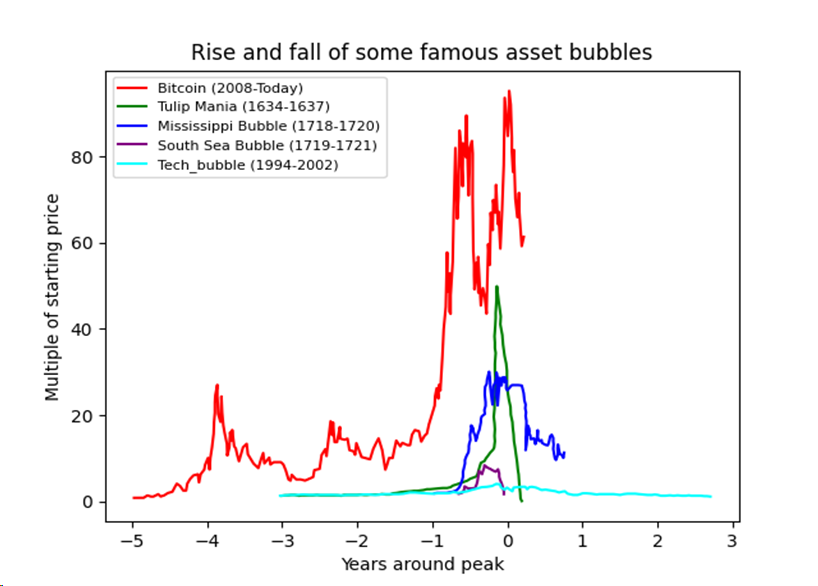
\includegraphics[width=0.6\linewidth]{Fig/01/F2}
    \caption{Bitcoin and Bubbles}
    \label{fig:f2}
\end{figure}
A major reason behind the popularity of Bitcoin is its strong security property, coupled with its truly decentralized nature. It is now well understood that as long as 51\% of the peers in Bitcoin are honest, the system is secure (the exact conditions are slightly different, but this suffices for the moment). This has been shown theoretically and has also been borne out in practice. Moreover, anyone can freely join and leave the Bitcoin system at any time; the system is \textbf{‘permissionless’}.\\\\
Some properties of Bitcoin and its performance are as follows:
\begin{enumerate}
    \item \textbf{Security}: We will discuss what it means when we say bitcoin is secure in future notes but generally, Bitcoin is secure as it is almost always accessible and it has never been broken.
    \item \textbf{Transaction throughputs}: Bitcoin has transaction of 7 tx/s which is noticeably low in amount. (See figure \ref{fig:f3})
    \item \textbf{Confirmation Latency }: Bitcoin has a very slow latency which can take hours before something gets confirmed.
    \item \textbf{Energy consumption}: Bitcoin and its mining are famous for their large energy consumption. It's that of a medium-sized country.
    \item \textbf{Computation and storage}: Mining bitcoin requires huge resources of computing and storage.
    \item \textbf{Communication}: Communication requirements are also fairly high. Everybody's transmitting everything and every possible message.
\end{enumerate}
Despite its benefits, there are major drawbacks of Bitcoin, which impact its viability. Some issues can be categorized as scaling issues. For example, the system can only process about seven transactions per second. In contrast, Visa (a centralized digital payment mechanism) processes 50,000 transactions per second. If all people in the world are to switch from Visa to Bitcoin, the system must ‘scale’ its transaction throughput. The rest of the issues are a lack of desirable properties. For instance, if the network is disrupted, transactions that were once ‘confirmed’ can be reverted. (We say that Bitcoin does not offer ‘finality’ in confirming transactions).
\begin{figure}[h!]
    \centering
    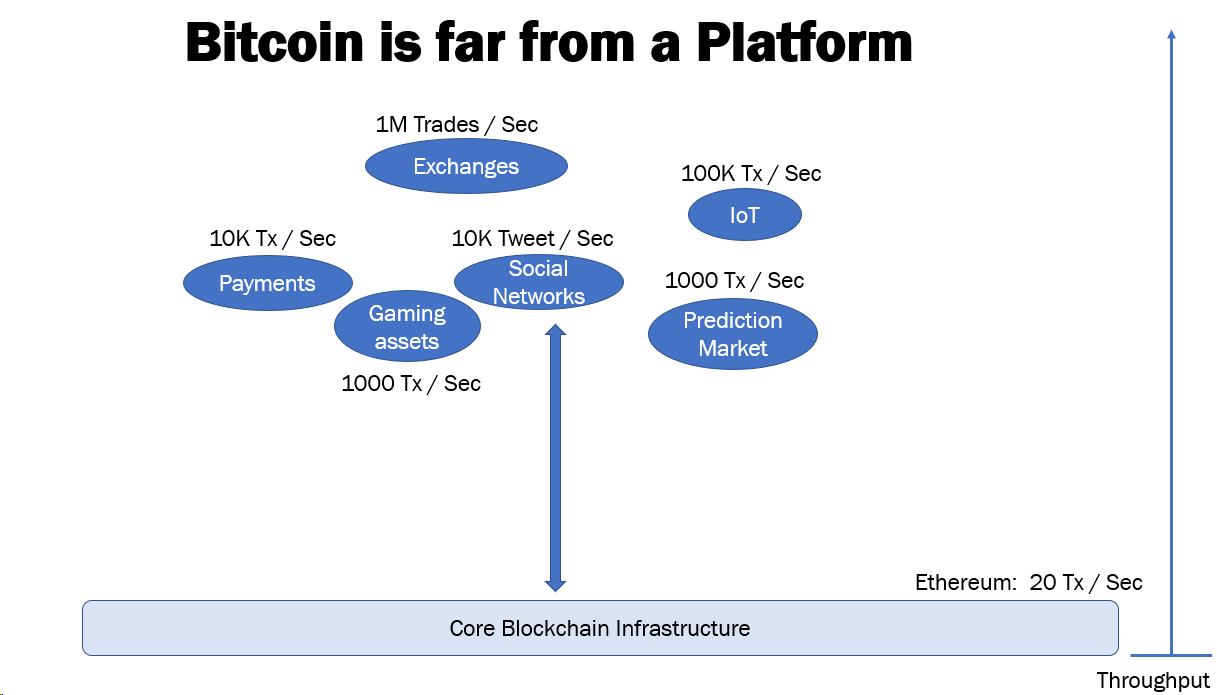
\includegraphics[width=0.8\linewidth]{Fig/01/F3}
    \caption{Evolution of Trust over human history}
    \label{fig:f3}
\end{figure}
\subsection*{Technical components}
\begin{itemize}
    \item \textbf{decentralized computer}:\\
    We are looking at basic libraries which include both networking libraries and cryptographic libraries. It mainly contains the followings:
    \begin{itemize}
        \item Cryptographic data structures
        \item Disk I/O, memory/cache and Database management
        \item Operating systems 
        \item Peer to peer networking
        \item Consensus and distributed algorithms
    \end{itemize}
    \item \textbf{Virtual machine}:
    \begin{itemize}
        \item \textbf{Reduced instruction set, incentives :} \\
        A virtual machine uses a simplified instruction set. It also has a decentralized structure that rewards each participant for their contribution, whether it is storage, computation, or data. This creates incentives at the instruction level, similar to how ants benefit from their collective work.
        \item \textbf{General purpose programming language} : \\
        A programming language can be built on top of this system.
    \end{itemize}
\end{itemize}
\subsection*{Technical challenges}
\begin{itemize}
    \item \textbf{Permissionless}:\\
    One of the main goals of designing a decentralized system is to achieve permissionless participation, where anyone can join and contribute to the network without requiring any authorization or intermediaries. However, this also poses a technical challenge, as the system needs to prevent spam and malicious behavior from adversaries who may try to disrupt or compromise the network.
    \item \textbf{Dynamic availability and safety}:\\
    Another goal is to ensure dynamic availability and safety, where the network can reach consensus and maintain its integrity even with the changing and unpredictable participation of nodes. This also requires a robust mechanism to deal with potential attacks from adversaries who may try to manipulate or censor the network.
    \item \textbf{Cryptography}:\\
    Cryptography provides some basic tools to address both of these design goals, such as digital signatures, hash functions, encryption, and zero-knowledge proofs. However, cryptography alone is not enough, as adversaries may also use sophisticated techniques to counter or exploit these tools. As the famous quote goes, "The trouble is, the other side can do magic too, Prime Minister." Therefore, designing a decentralized system requires a careful balance of cryptography, incentives, game theory, and distributed algorithms.
\end{itemize}

\section{What this course is about}
This course covers the \textbf{fundamental design principles of blockchains}. We aim to look at good blockchain designs as a full computer rather than isolated elements (we are not going to look only at cryptography parts or algorithm parts, etc.).
Basic background in algorithms, probability, system programming skills (C/C++) and maturity in nearly all aspects of computer science are required and will be used.\\\\
The lectures are divided into three modules:
\begin{enumerate}
    \item \textbf{Understanding Bitcoin}\\
    The first six lectures cover the complete design of Bitcoin. At the end of this module, you will be able to understand the system as a whole and how it functions as a  secure, decentralized payment platform. We will introduce various terms about Bitcoin and cryptocurrencies (e.g., UTXOs, hash pointers, longest chain rule) and cryptography on a “need-to-know basis.” We will study some attacks on Bitcoin and under what conditions Bitcoin is secure under those attacks.
    \item \textbf{Scaling Bitcoin}\\
    The second module aims to improve the throughput, latency, and resource usage
    (energy, compute, storage, and communication needs) of Bitcoin while maintaining the same security
    levels. The goal is to work within the overall architecture of Bitcoin itself and systematically improve
    various design elements.
    \item \textbf{Beyond Bitcoin}\\
    The third module covers alternate blockchain protocols that offer properties
    that are simply not present in Bitcoin. These include accountability, resistance to 51\% adversarial
    attacks, transaction finality, and privacy (the exact meaning of these terms will be made clear later
    on). We also see how these properties can be combined with Bitcoin-like blockchains via the notion
    of a ‘finality gadget.’ This gives us a blockchain with many desirable properties.
\end{enumerate}
This course emphasizes the implementation of blockchains (in software).
Thus, the bulk of the evaluation will be based on two projects. The first project involves implementing
a Bitcoin client. This will make use of all the concepts learned in the first module of the course.
The second project will involve implementing a finality gadget of your choice on top of Bitcoin (from
the third module). Rust will be the programming language that is used.

\section{What is Rust?}
Rust is a compiled language such as C and C++ and is built for reliability. In Rust, we have runtime and compile time safety together and it helps to have memory and thread safety. This is very important in blockchain. In general, when a language or model is agreed upon in the blockchain, changing it is indistinguishable from a security attack. Therefore, when the differential method is done, the blockchain cannot be changed or is very difficult to change. Therefore, unlike other applications in the blockchain, it is not easy to add new code and new changes.\\ For example, the changes that took place in Ethereum took several years because, in addition to the above, it was necessary for all participants to vote, take a stand, and move toward the changes. Therefore, the blockchain program must be well written, and for this reason, rust is used.
